\chapter{Modelagem FrameWeb}
\label{sec-frameweb}
\vspace{-1cm}

\emph{\imprimirtitulo} é um sistema Web cuja arquitetura utiliza \textit{frameworks} comuns no desenvolvimento para esta plataforma. Desta forma, o sistema pode ser modelado utilizando a abordagem FrameWeb~\cite{souza-celebratingfalbo20}.

A Tabela~\ref{tabela-frameworks} indica os \textit{frameworks} presentes na arquitetura do sistema que se encaixam em cada uma das categorias de \textit{frameworks} que FrameWeb dá suporte. Em seguida, os modelos FrameWeb são apresentados para cada camada da arquitetura.

\begin{footnotesize}
	\begin{longtable}{|c|c|}
		\caption{\textit{Frameworks} da arquitetura do sistema separados por categoria.}
		\label{tabela-frameworks}\\\hline
		
		\rowcolor{lightgray}
		\textbf{Categoria de \textit{Framework}} & \textbf{\textit{Framework} Utilizado} \\\hline 
		\endfirsthead
		\hline
		\rowcolor{lightgray}
		\textbf{Categoria de \textit{Framework}} & \textbf{\textit{Framework} Utilizado} \\\hline 
		\endhead

		Controlador Frontal & Flask \\\hline

		Injeção de Dependências & Flask (Blueprints e extensões) \\\hline

		Mapeamento Objeto/Relacional & SQLAlchemy \\\hline

		Segurança & Flask Security \\\hline
	\end{longtable}
\end{footnotesize}

\section{Camada de Negócio}
\label{sec-frameweb-negocio}

\begin{figure}[H]
	\centering
	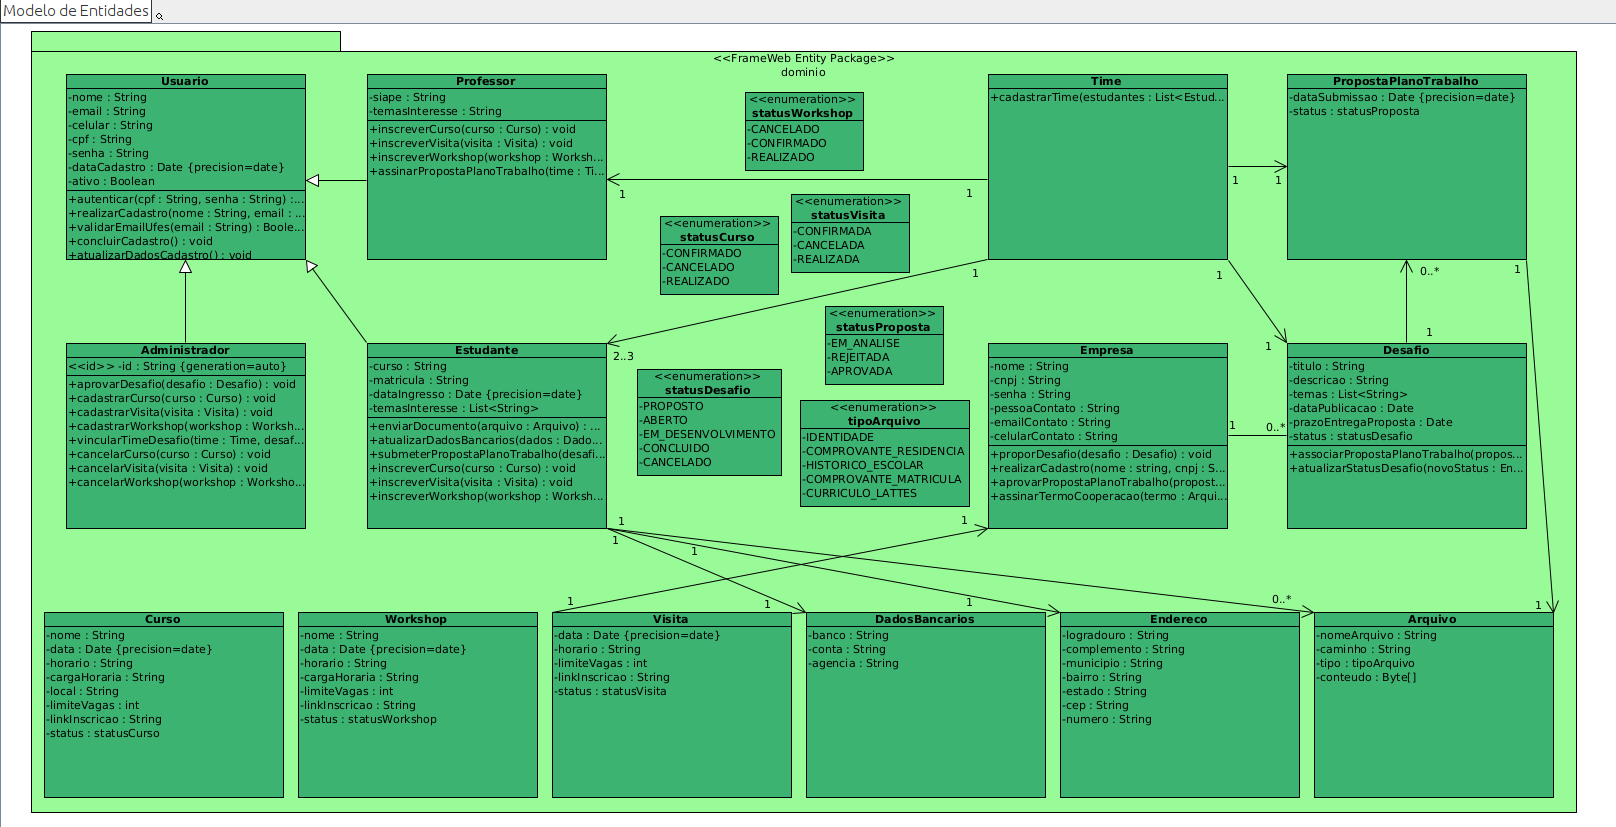
\includegraphics[width=1.0\textwidth]{figuras/figura_modelo_entidades.png}
	\caption{Modelo de entidades do FrameWeb.}
	\label{figura-entidades}
\end{figure}

Este sistema modela a interação entre estudantes, empresas e administradores em uma plataforma de desenvolvimento profissional.

O fluxo principal envolve Empresas que propõem Desafios (projetos), para os quais Estudantes podem se organizar em Times e submeter Propostas de Trabalho. Essa relação estabelece o principal ciclo de colaboração da plataforma.

Paralelamente, Administradores são responsáveis por gerenciar o sistema e organizar eventos como Cursos, Workshops e Visitas. Os estudantes podem se inscrever e participar dessas atividades para complementar sua formação. O modelo também inclui entidades de suporte para gerenciar dados como Endereços, Dados Bancários e Arquivos, além de utilizar status para controlar o andamento de todas as atividades, desde a aprovação de uma proposta até a realização de um evento.

\begin{figure}[H]
	\centering
	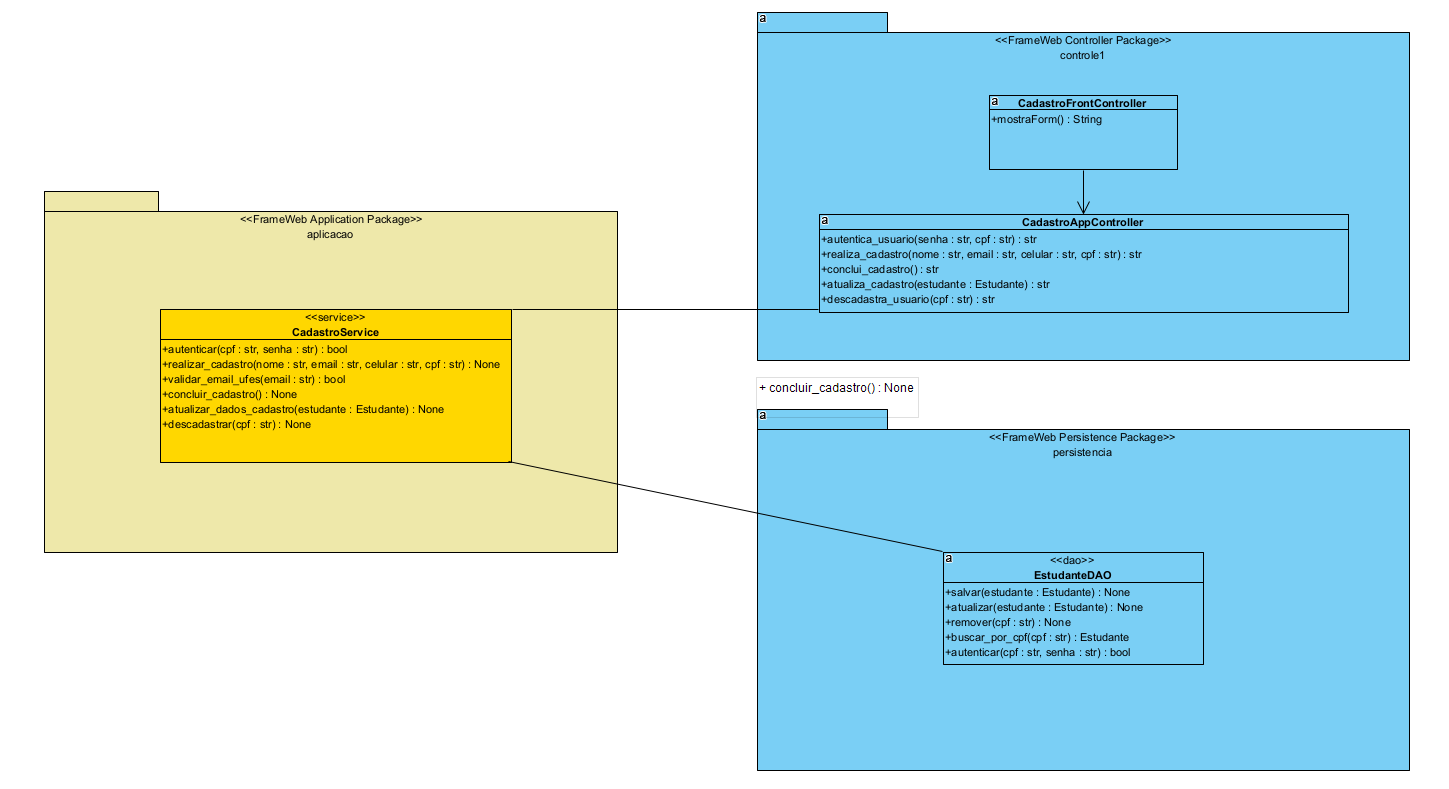
\includegraphics[width=1.0\textwidth]{figuras/figura_modelo_aplicacao.png}
	\caption{Modelo de aplicação do FrameWeb: Cadastro de Estudantes.}
	\label{figura-aplicacao}
\end{figure}

Este diagrama descreve a arquitetura de software para a funcionalidade de cadastro, organizada em três camadas distintas para separar responsabilidades e organizar o código.

O fluxo se inicia na camada de Controle, onde a classe `CadastroAppController` recebe os dados enviados pelo usuário. Esta camada atua como a porta de entrada, recebendo a requisição e delegando-a para a camada de serviço para o devido processamento.

Em seguida, a requisição é tratada pela camada de Aplicação. Nela, a classe `CadastroService` é responsável por executar a lógica de negócio central. É sua função realizar as validações necessárias, como a de um e-mail ou CPF, para garantir a integridade dos dados antes de registrar o usuário no sistema.

Finalmente, após a validação, a camada de serviço aciona a camada de Persistência. A classe `EstudanteDAO` (Data Access Object) tem a função exclusiva de se comunicar com o banco de dados para realizar as operações de salvar, atualizar ou buscar as informações do estudante. Essa estrutura garante que as regras de negócio permaneçam independentes do acesso a dados e da interface com o usuário.

\section{Camada de Acesso a Dados}
\label{sec-frameweb-dados}

\begin{figure}[H]
	\centering
	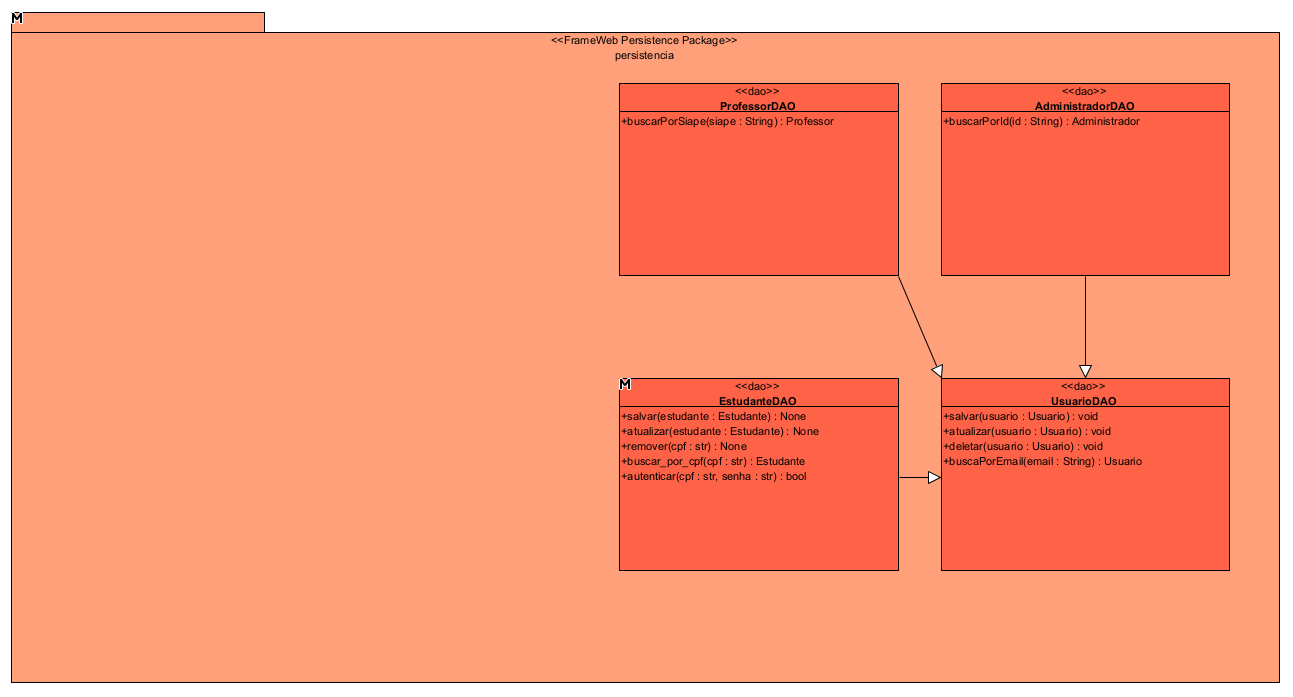
\includegraphics[width=1.0\textwidth]{figuras/figura_modelo_persistencia.png}
	\caption{Modelo de persistência do FrameWeb: Usuário.}
	\label{figura-persistencia}
\end{figure}

Este diagrama detalha a arquitetura da camada de persistência do sistema, mostrando como as classes do tipo DAO (Data Access Object) são organizadas para interagir com o banco de dados. O objetivo principal destas classes é gerenciar o salvamento, a atualização, a busca e a remoção das informações de cada tipo de usuário.

A estrutura é centralizada na classe base `UsuarioDAO`, que define as operações comuns a todos os usuários do sistema. Ela contém métodos genéricos para salvar, atualizar, deletar e buscar um usuário por e-mail. Esta classe serve como um contrato fundamental para a persistência de qualquer entidade do tipo usuário, promovendo a reutilização de código.

A partir desta base, outras classes especializadas herdam suas funcionalidades. O `EstudanteDAO`, `AdministradorDAO` e `ProfessorDAO` são especializações que, além de possuírem todas as operações do `UsuarioDAO`, adicionam métodos específicos para suas respectivas entidades. Por exemplo, o `EstudanteDAO` inclui métodos para buscar por CPF e autenticar, enquanto o `ProfessorDAO` permite a busca por Siape. Essa abordagem de herança cria um modelo de acesso a dados que é ao mesmo tempo robusto, centralizado e flexível para atender às necessidades de cada tipo de usuário.

\section{Camada de Apresentação}
\label{sec-frameweb-apresentacao}

\begin{figure}[H]
	\centering
	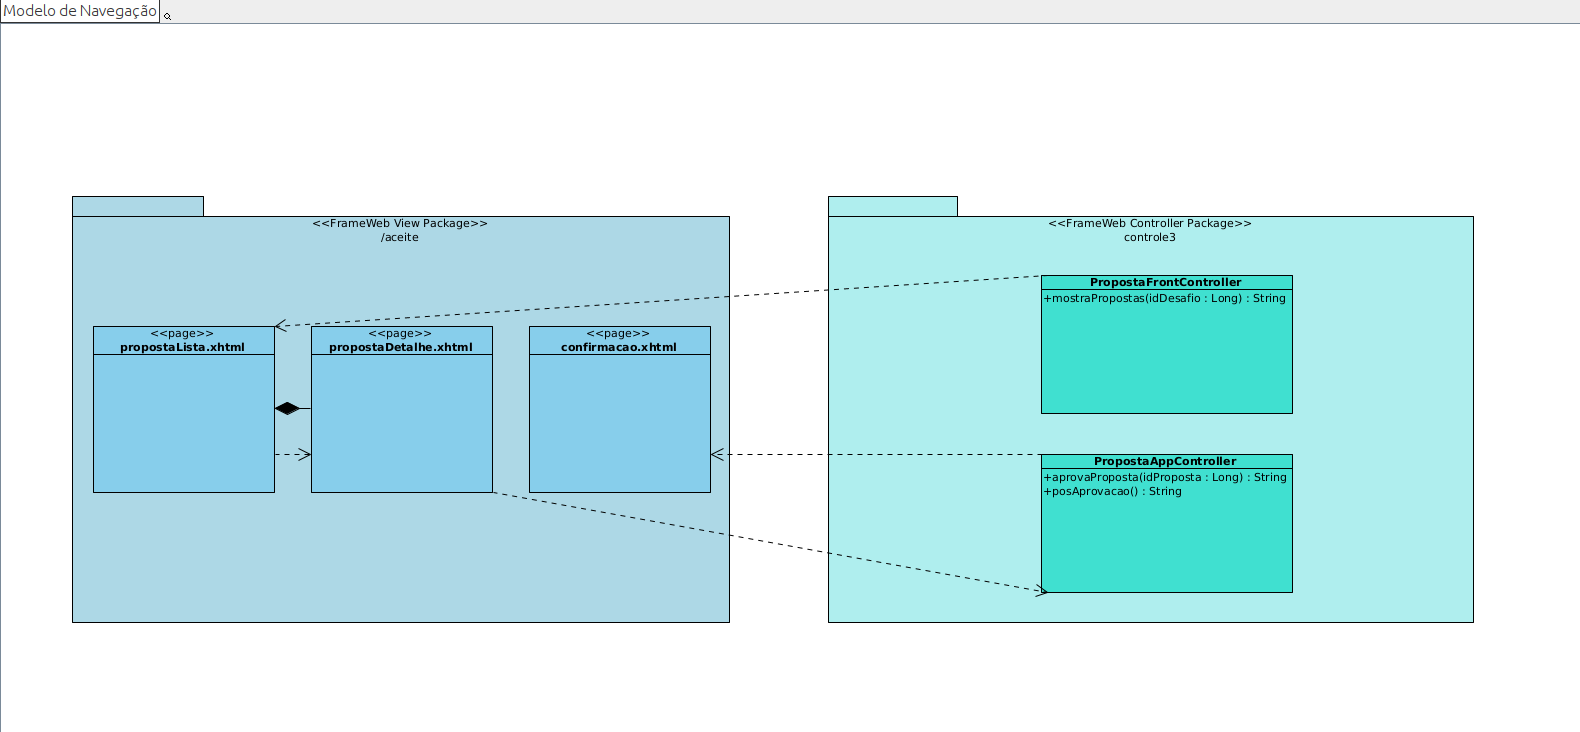
\includegraphics[width=1.0\textwidth]{figuras/figura_modelo_navegacao_cadastro.png}
	\caption{Modelo de navegação do FrameWeb - Cadastro.}
	\label{figura-cadastro}
\end{figure}

Este modelo de Cadastro detalha a navegação do usuário durante o processo de cadastro no sistema. O fluxo se inicia quando o CadastroFrontController direciona o usuário para a página principal de cadastro, a cadastroForm.xhtml. Ao preencher e submeter o formulário, a ação concluiCadastro é acionada no CadastroAppController, que processa os dados. Após o processamento, o sistema pode navegar o usuário para diferentes páginas, dependendo do resultado. Em caso de sucesso, o usuário é levado para a tela cadastroConcluido.xhtml. O fluxo também prevê etapas adicionais, como as páginas completaPerfil.xhtml e confirmaEmail.xhtml. O modelo também inclui um fluxo de atualização de dados, onde a página cadastroEstudante.xhtml permite acionar a ação atualizaCadastro, e uma página de erro, cadastroErro.xhtml, para lidar com possíveis falhas.

\begin{figure}[H]
	\centering
	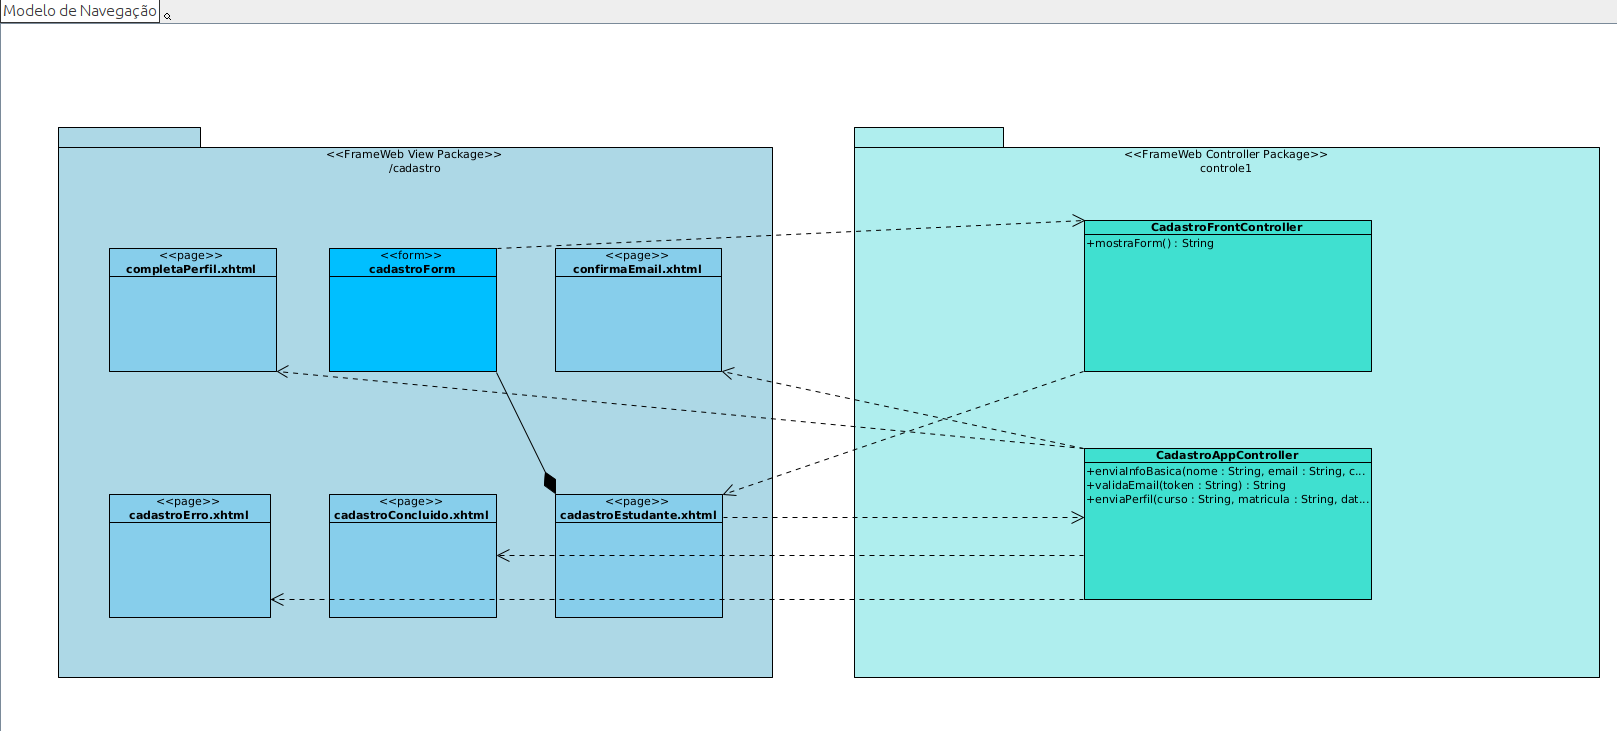
\includegraphics[width=1.0\textwidth]{figuras/figura_modelo_navegacao_notificacao.png}
	\caption{Modelo de navegação do FrameWeb - Notificação.}
	\label{figura-notificacao}
\end{figure}

Este modelo de Notificação descreve o fluxo de navegação para a análise e o aceite de propostas. O processo começa quando o PropostaFrontController exibe a lista de propostas disponíveis na página propostaLista.xhtml. A partir desta lista, o usuário pode selecionar uma proposta para visualizar seus detalhes, sendo direcionado para a página propostaDetalhe.xhtml. Na tela de detalhes, o usuário tem a opção de aprovar a proposta, o que aciona o método aprovaProposta no PropostaAppController. Uma vez que a ação de aprovação é processada com sucesso no sistema, o controlador executa a lógica de posAprovacao, que finaliza o fluxo redirecionando o usuário para a página confirmacao.xhtml, informando sobre o sucesso da operação.

\begin{figure}[H]
	\centering
	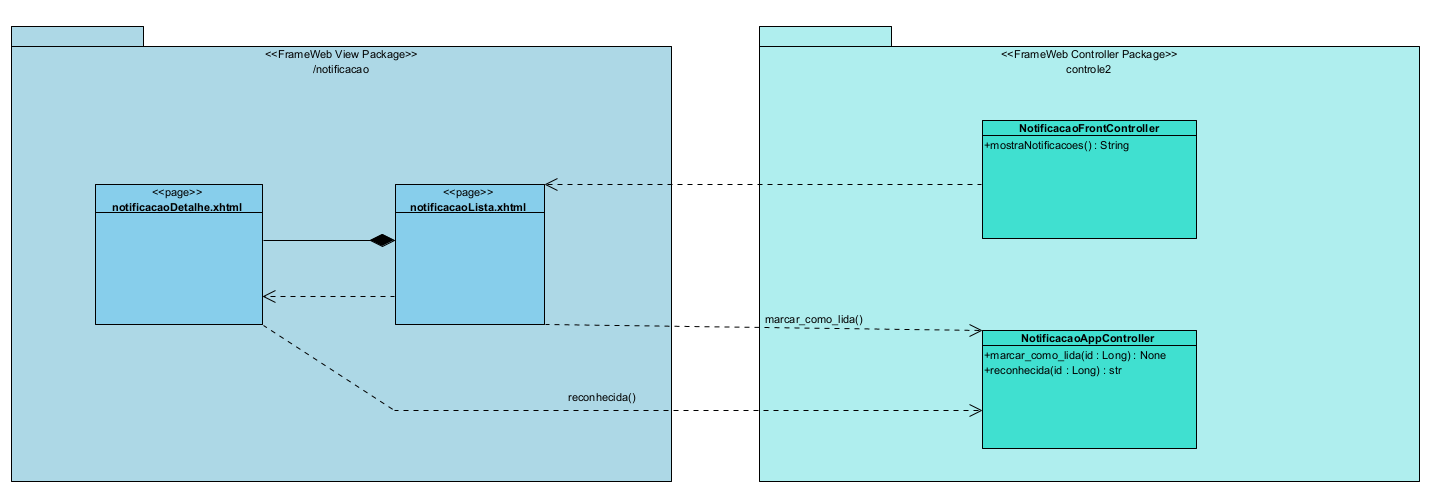
\includegraphics[width=1.0\textwidth]{figuras/figura_modelo_navegacao_aceite.png}
	\caption{Modelo de navegação do FrameWeb - Aceite.}
	\label{figura-aceite}
\end{figure}

Este modelo de Aceite ilustra o fluxo de navegação do usuário ao interagir com o sistema de notificações. O fluxo se inicia com o NotificacaoFrontController, que é responsável por exibir a lista de notificações na página notificacaoLista.xhtml. A partir desta tela, o usuário pode clicar em uma notificação para ser levado à página notificacaoDetalhe.xhtml. Na página de detalhes, o usuário pode interagir com a notificação. Ele pode executar a ação marcarComoLida, que atualiza o status da notificação no sistema, ou acionar a ação reconhecida. Esta última, ao ser processada pelo NotificacaoAppController, efetua um redirecionamento, navegando o usuário para uma nova página e concluindo a interação com aquela notificação específica.







